\documentclass{article}

\usepackage[utf8]{inputenc} % accents
\usepackage[T1]{fontenc}      % caractères français
\usepackage{geometry}         % marges
\usepackage[francais]{babel}  % langue
\usepackage{graphicx}         % images
\usepackage{verbatim}
\usepackage{url}
\bibliographystyle{alpha}

\title{Document d'analyse des besoins}
\author{Alexandre Casanova-Franger\\
        \and
        Gauthier Lamarque\\
        \and
        Paul Simorre\\
        \and
        Lucas Vivas\\}

\begin{document}
  \maketitle
  \section{Introduction}
    \paragraph{}
    Ce projet consiste à réaliser un outil informatique d'analyse musicale dans
    l'optique de faciliter l'improvisation. À terme, cet outil aura pour
    objectif de permettre à des musiciens de pouvoir se calibrer sur les membres
    qui jouent le mieux ensemble. De plus, cet outil aura une portée
    scientifique, dans le sens où il sera possible d'étudier l'adaptation des
    musiciens grâce au retours fournis par l'outil. \\
    Cet outil est basé sur une plateforme externe appelée Bela \cite{BELA},
    qui est un système embarqué de traitement audio en temps réel.
  \section{Description et analyse de l'existant}
    \paragraph{}
    À ce jour, l'outil est capable de fournir une représentation graphique de la
    corrélation des entrées audio. Ces entrées sont représentées par des
    tableaux. Une fonction prenant ces tableaux en entrée
    retourne un nombre flottant compris entre 0 et 1, et qui représente la
    corrélation entre les deux entrées. Pour n entrées, la représentation sera
    donc une matrice carrée de taille n.\\
    Dans un souci d'évolution, il est possible d'ajouter de nouvelles fonctions
    de calcul de corrélation. Il suffit de respecter une signature de méthode,
    et de placer les fichiers sources dans le dossier prévu à cet effet.\\
  \section{Description des besoins}
    \subsection{Besoins fonctionnels}
    \paragraph{}
    \begin{itemize}
      \item L'utilisateur pourra avoir un retour sonore qui dépendra de la
      matrice de corrélation et d'une configuration,
      \item L'utilisateur pourra avoir une représentation graphique des niveaux
      sonores sous la forme d'une matrice, de la même manière que la matrice de
      corrélation.
      \item L'utilisateur aura à sa disposition une liste de configurations
      pré-établies, dont les suivantes :
      \begin{itemize}
        \item Augmenter le volume des paires d'entrées les plus corrélées
        \item Augmenter le volume des paires d'entrées les moins corrélées
        \item Augmenter le volumes des entrées dont la somme des indices de
        corrélation avec toutes les autres entrées est la plus élevée.
      \end{itemize}
      \item L'utilisateur pourra ajouter une nouvelle configuration, suivant
      une signature donnée.
      \item L'utilisateur pourra changer la fenêtre temporelle de calcul de
      corrélation.
    \end{itemize}
    \subsection{Besoins non-fonctionnels}
    \begin{itemize}
      \item Les signatures des méthodes calculant les niveaux sonores des
      entrées devront être génériques de façon à permettre aux utilisateurs d'en
      ajouter de nouvelles.
      \item Le temps de latence du programme doit être inférieur à 1 seconde.
      En effet, la durée d'acquisition de données (delta t) sera de 1 seconde,
      donc si l'on veut donner un sortie audio en temps réel, il faut que la latence
      soit au maximum de 1 seconde.
    \end{itemize}
    \subsection{Scénarios, prototypes, diagrammes, etc.}
      \paragraph{}
      Nous allons décrire ci-après un scénario que nos clients ont imaginé :\\
      L'utilisateur utilisa l'outil sur un groupe de musiciens. Des micros sont
      branchés sur les différents entrées analogiques et chaque musicien dispose
      d'un retour son. L'utilisateur configure le fichier de confguration afin
      que les paramètres décrits ci-dessus soient correctement pris en compte
      par l'outil. Les musiciens se mettent à improviser comme bon leur semble,
      et l'on peut observer en temps réel les corrélations entre les différents
      musiciens. On pourra aussi observer une matrice dite de "mixage" qui
      affiche les différents poids des paires de musiciens en fonction d'une
      configuration par défaut. À tout moment, l'utilisateur peut choisir une
      configuration de mixage différente pour que le retour sonore change.\\
      L'intérêt est d'étudier comment les musiciens s'adaptent en fonction du
      retour sonore, donc en fonction de la configuration de mixage choisie.
  \section{Diagramme de Gantt}
    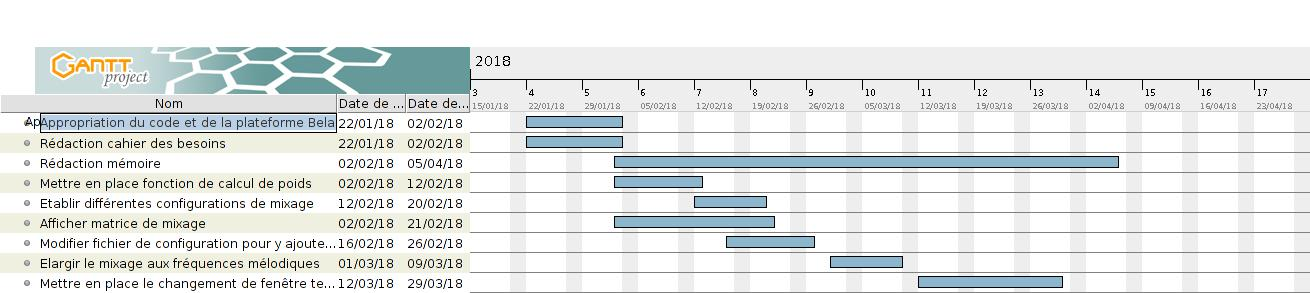
\includegraphics[scale=0.35]{DiagrammeAnalyseBesoins.jpg}
  \bibliography{analyse-besoins}
\end{document}
